\chapter{Pruebas}

Según la metodología ``cascada'', la fase de implementación se cierra cuando se realizan las pruebas respectivas sobre los módulos que se implementaron. Para probar en su totalidad el sistema de video-vigilancia se plantean las siguientes pruebas de aceptación.\\

\section{Prueba de conexión del módulo de cámaras}
En la tabla \ref{con_modulo_cameras} se detalla la prueba realizadas de conexión del módulo de cámaras.

\begin{table}[H]
    \caption{Prueba de conexión en módulo de cámaras}
    \label{con_modulo_cameras}
    \begin{center}
        \begin{tabular}{|>{\centering}p{0.3\textwidth}|m{0.6\textwidth}<{\centering}|} 
            \hline
            \textbf{Título de la prueba} & \textbf{Única cámara conectada} \\
            \hline
            \textbf{Descripción} & El servidor se encuentra en ejecución y una instancia del módulo de cámaras se conecta al servidor. No existen más cámaras conectadas.\\
            \hline
            \textbf{Comportamiento obtenido} & 
            \begin{itemize}
                \item El servidor registra la desconexión y lo muestra en consola.
                \item El servidor notifica al usuario por medio de correo electronico.
                \item La notificación provee información sobre la fecha y hora de la desconexión.
                \item La notificación detalla que no hay más conexiones.
            \end{itemize} \\ 
            \hline
            \textbf{Estado de prueba} & Exitoso \\
            \hline
        \end{tabular}
        \begin{center}
            Fuente: Elaboración propia.
        \end{center}
    \end{center}
\end{table}

El módulo del servidor se encuentra a la espera de nuevas conexiones y en la figura \ref{camera_connected_one_camera} se visualiza los mensajes que se muestran el la interfaz del servidor a partir del comportamiento esperado del módulo.\\

\begin{figure}[H]
    \begin{center}
        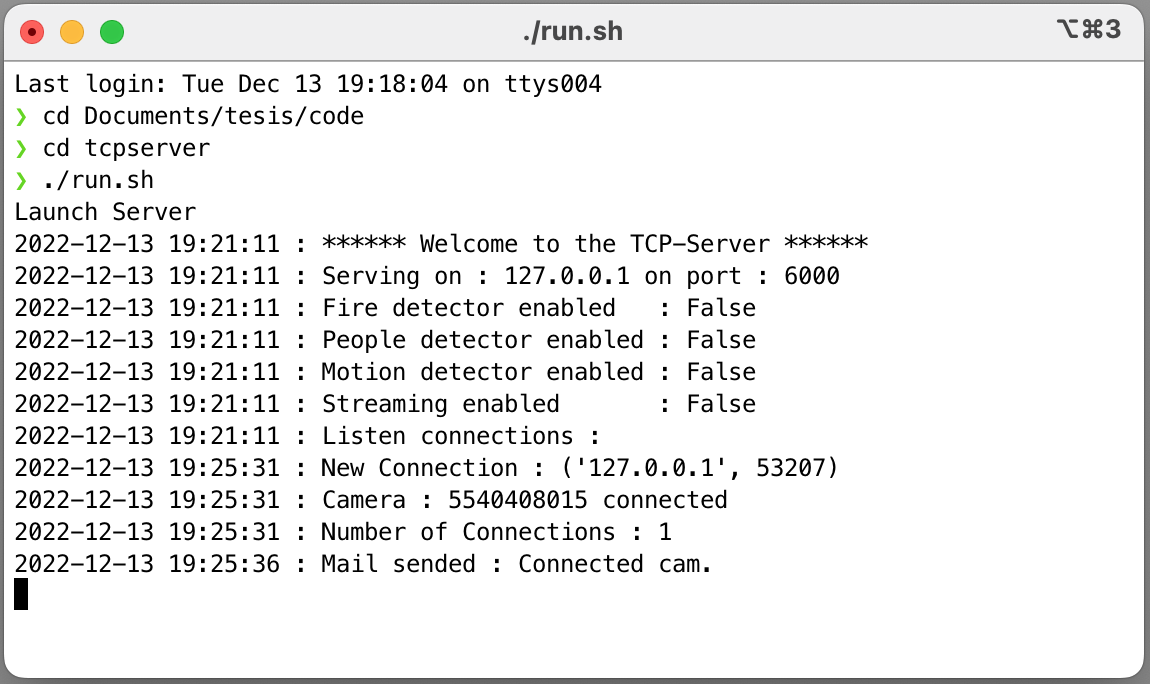
\includegraphics[width=13cm]{img/capitulo_6/server_cam_connected.png}
    \end{center}
    \begin{center}
        \caption{Mensajes de la interfaz del servidor.}
        Fuente : Elaboración propia
        \label{camera_connected_one_camera}
    \end{center}
\end{figure}

En la figura \ref{mail_one_camera_connected} se visualiza el correo electrónico que el usuario recibe como notificación despues de que una cámara se conecta al sistema.\\

\begin{figure}[H]
    \begin{center}
        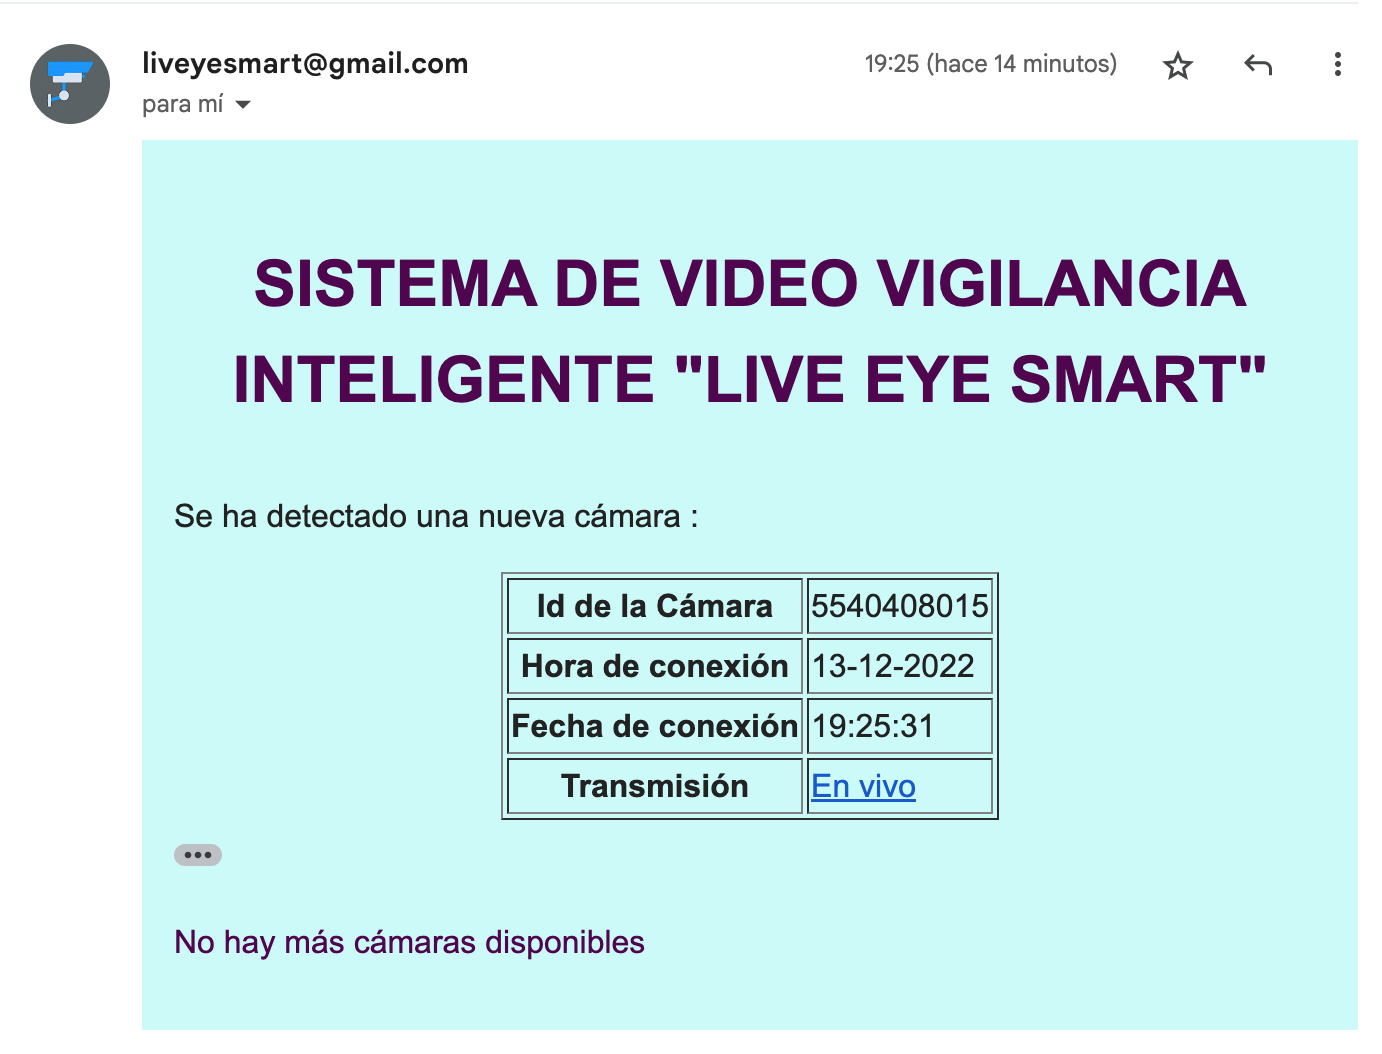
\includegraphics[width=12cm]{img/capitulo_6/mail1.png}
    \end{center}
    \begin{center}
        \caption{Notificación por correo - Una cámara conectada.}
        Fuente : Elaboración propia
        \label{mail_one_camera_connected}
    \end{center}
\end{figure}

En la tabla \ref{many_cameras_connected_table} se detalla el caso cuando se tiene varias cámaras conectadas y se conecta una cámara adicional.\\

\begin{table}[H]
    \caption{Conexión de varias cámaras}
    \begin{center}
        \begin{tabular}{|>{\centering}p{0.3\textwidth}|m{0.6\textwidth}<{\centering}|} 
            \hline
            \textbf{Título de la prueba} & Más de una cámara conectada \\
            \hline
            \textbf{Descripción} & El servidor se encuentra en ejecución y una instancia del módulo de cámaras se conecta al servidor. Existen más de una cámara conectada.\\
            \hline
            \textbf{Comportamiento obtenido} & 
            \begin{itemize}
                \item El servidor acepta la conexión y lo muestra en consola.
                \item El servidor notifica al usuario por medio de correo electronico.
                \item La notificación provee información sobre la fecha y hora de la conexión, compartiendo el enlace para la transmisión en vivo.
                \item La notificación provee la misma información de las demás cámaras conectadas al servidor.
            \end{itemize} \\ 
            \hline
            \textbf{Estado de prueba} & Exitoso \\
            \hline
        \end{tabular}
        \label{many_cameras_connected_table}
        \begin{center}
            Fuente: Elaboración propia.
        \end{center}
    \end{center}
\end{table}

A continuación se muestra capturas del comportamiento esperado:

\begin{figure}[H]
    \begin{center}
        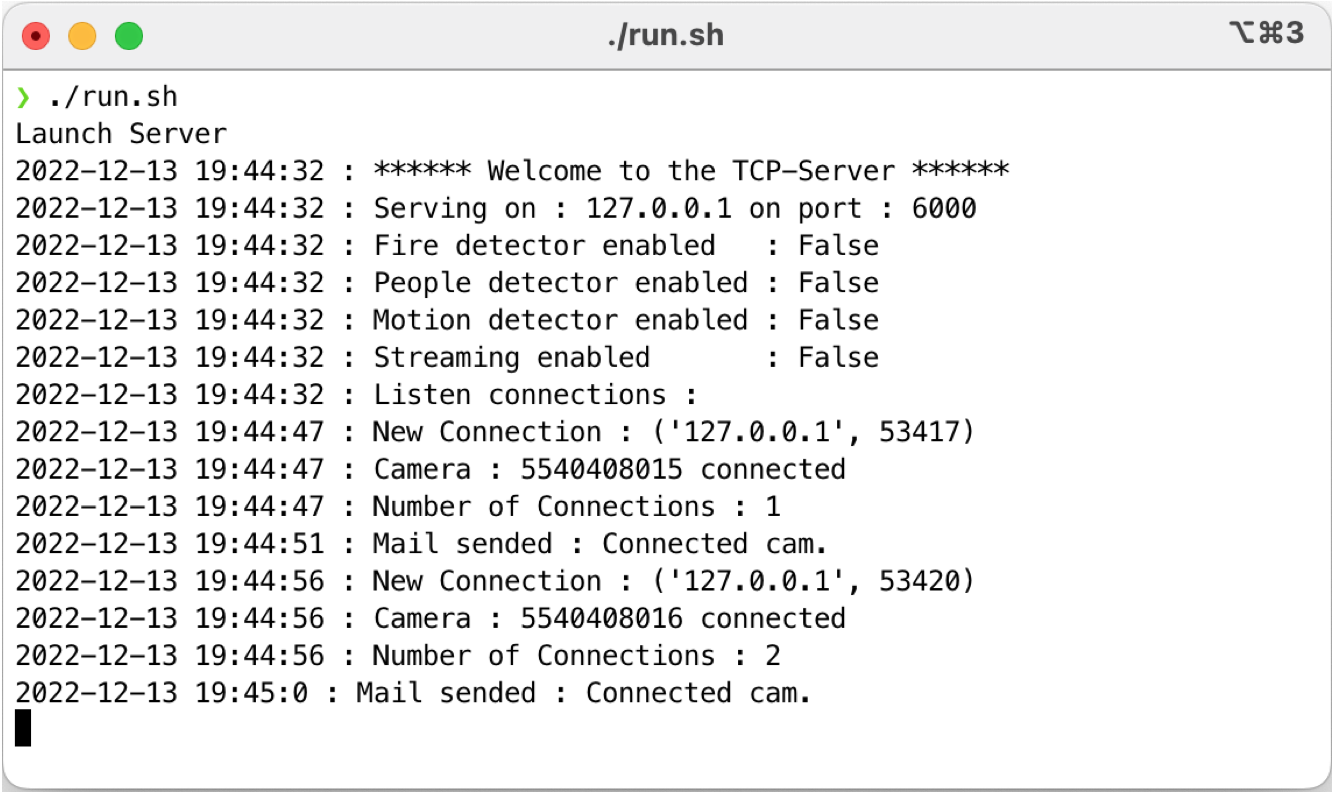
\includegraphics[width=12cm]{img/capitulo_6/server_cam_connected_more_cams.png}
    \end{center}
    \begin{center}
        \caption{Mensajes en consola del servidor - Más de una cámara conectada.}
        Fuente : Elaboración propia
    \end{center}
\end{figure}

\begin{figure}[H]
    \begin{center}
        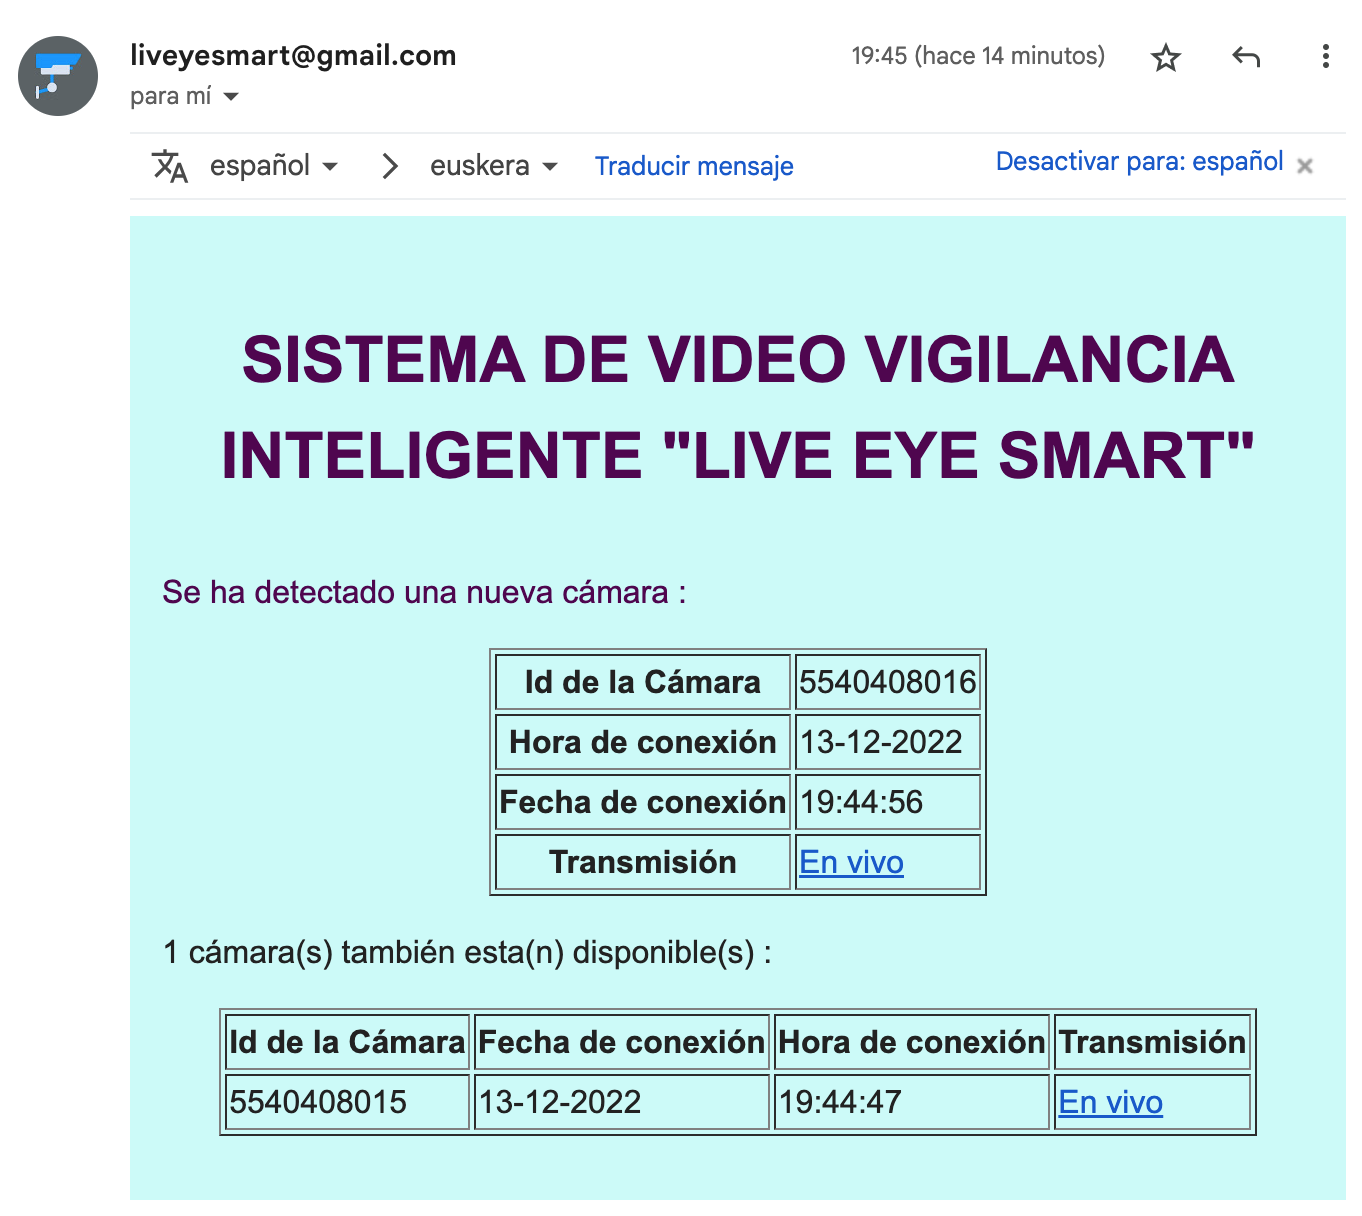
\includegraphics[width=10cm]{img/capitulo_6/mail2.png}
    \end{center}
    \begin{center}
        \caption{Notificación por correo - Más de una cámara conectada.}
        Fuente : Elaboración propia
    \end{center}
\end{figure}


\section{Prueba de desconexión del módulo de cámaras}

En la siguiente tabla se describe una de las pruebas realizadas:

\begin{table}[H]
    \caption{Detalle de prueba de desconexión del módulo de cámaras, única cámara conectada}
    \begin{center}
        \begin{tabular}{|>{\centering}p{0.3\textwidth}|m{0.6\textwidth}<{\centering}|} 
            \hline
            \textbf{Título de la prueba} & Única cámara conectada y se desconecta \\
            \hline
            \textbf{Descripción} & El servidor se encuentra en ejecución y la única instancia del módulo de cámaras se desconecta del servidor. No existen más cámaras conectadas.\\
            \hline
            \textbf{Comportamiento obtenido} & 
            \begin{itemize}
                \item El servidor registra la desconexión y lo muestra en consola.
                \item El servidor notifica al usuario por medio de correo electronico.
                \item La notificación provee información sobre la fecha y hora de la desconexión.
                \item La notificación detalla que no hay más conexiones.
            \end{itemize} \\ 
            \hline
            \textbf{Estado de prueba} & Exitoso \\
            \hline
        \end{tabular}
    \end{center}
    \begin{center}
        Fuente: Elaboración propia.
    \end{center}
\end{table}

A continuación se muestra capturas del comportamiento esperado:

\begin{figure}[H]
    \begin{center}
        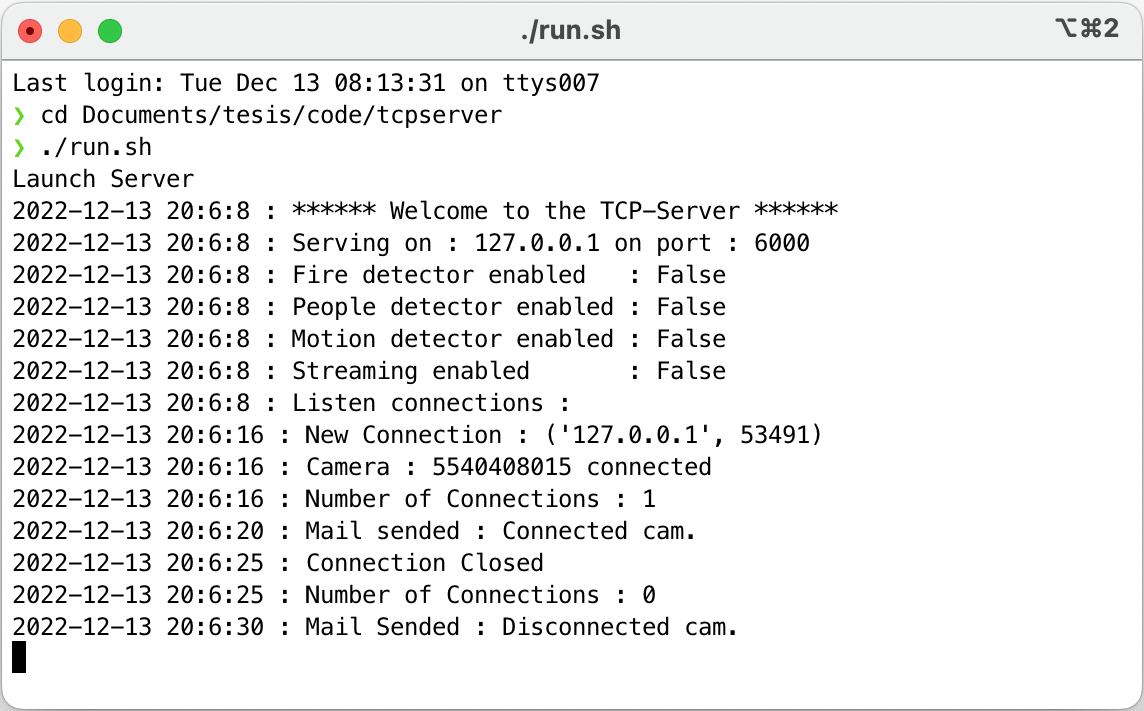
\includegraphics[width=12cm]{img/capitulo_6/cam_disconnected_1_cam.png}
    \end{center}
    \begin{center}
        \caption{Mensajes en consola del servidor - Única cámara desconectada.}
        Fuente : Elaboración propia
    \end{center}
\end{figure}

\begin{figure}[H]
    \begin{center}
        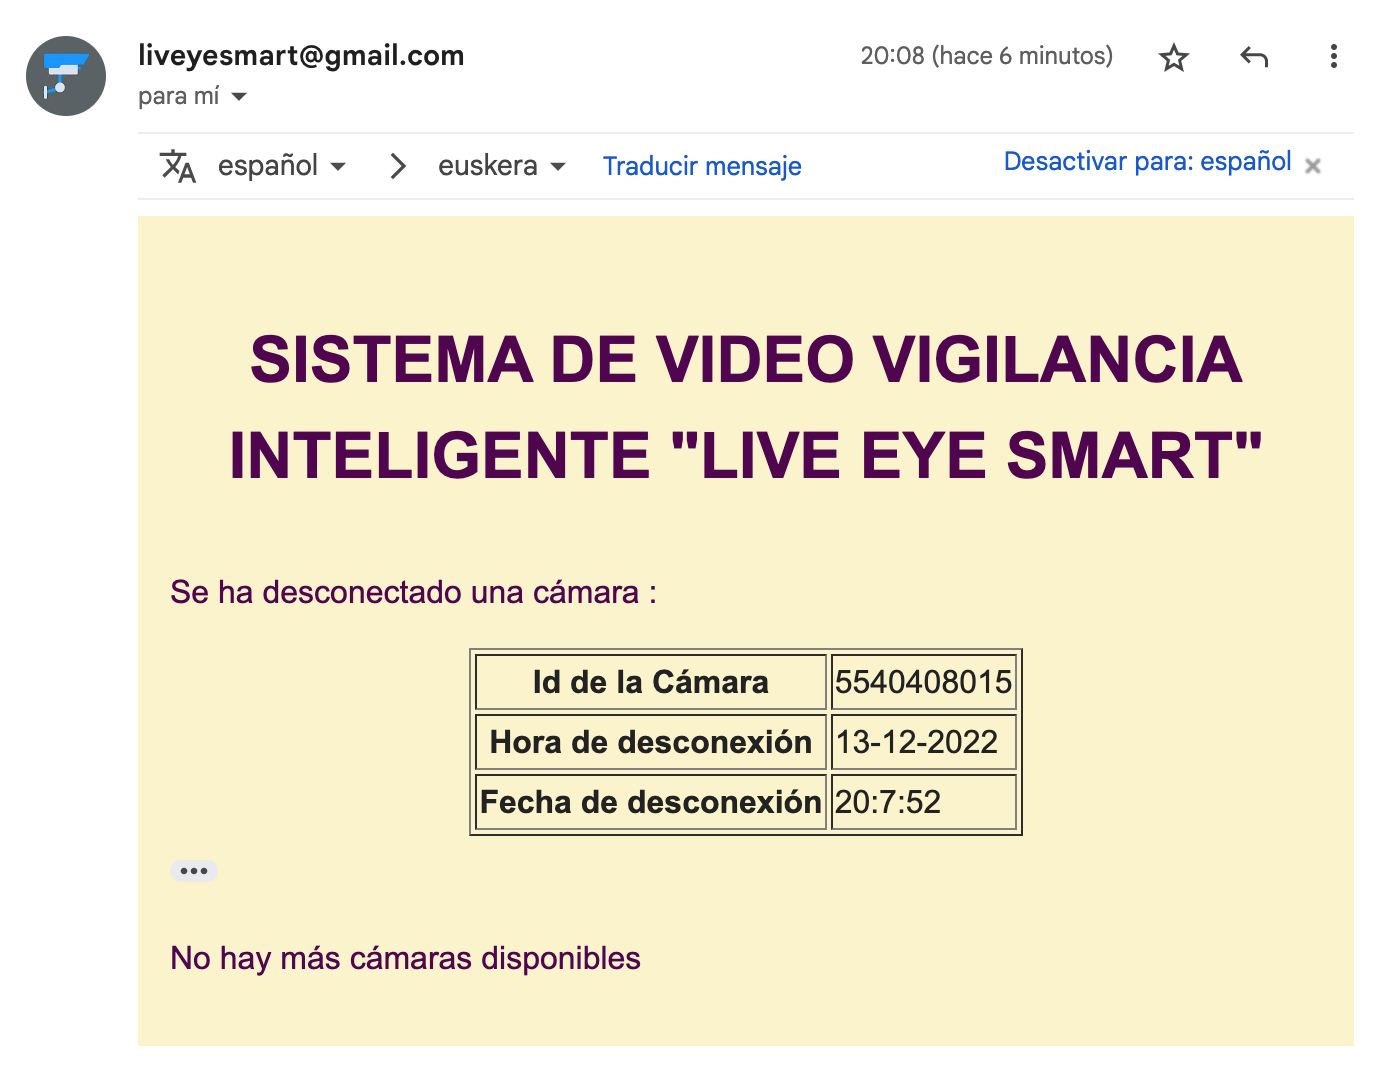
\includegraphics[width=12cm]{img/capitulo_6/mail4.png}
    \end{center}
    \begin{center}
        \caption{Notificación por correo - Única cámara desconectada.}
        Fuente : Elaboración propia
    \end{center}
\end{figure}

En la siguiente tabla se describe otra de las pruebas realizadas:\\

\begin{table}[H]
    \caption{Detalle de prueba de desconexión de módulo de cámaras con más de una cámara conectada}
    \begin{center}
        \begin{tabular}{|>{\centering}p{0.3\textwidth}|m{0.6\textwidth}<{\centering}|} 
            \hline
            \textbf{Título de la prueba} & Una de las cámaras es desconectada \\
            \hline
            \textbf{Descripción} & El servidor se encuentra en ejecución y una instancia del módulo de cámaras se desconecta del servidor. Existen más cámaras conectadas.\\
            \hline
            \textbf{Comportamiento obtenido} & 
            \begin{itemize}
                \item El servidor acepta la conexión y lo muestra en consola.
                \item El servidor notifica al usuario por medio de correo electronico.
                \item La notificación provee información sobre la fecha y hora de la conexión, compartiendo el enlace para la transmisión en vivo.
            \end{itemize} \\ 
            \hline
            \textbf{Estado de prueba} & Exitoso \\
            \hline
        \end{tabular}
    \end{center}
    \begin{center}
        Fuente: Elaboración propia.
    \end{center}    
\end{table}

A continuación se muestra capturas del comportamiento esperado:

\begin{figure}[H]
    \begin{center}
        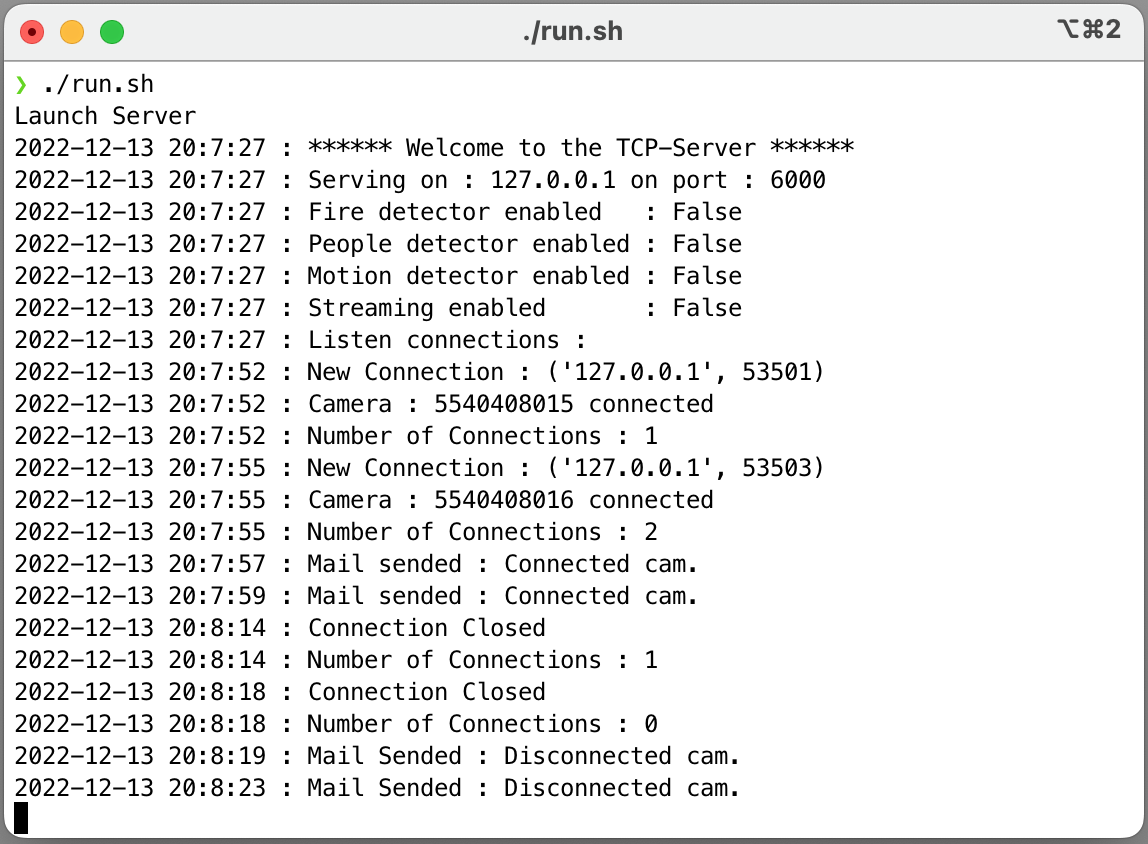
\includegraphics[width=13cm]{img/capitulo_6/cam_disconnected_n_cams.png}
    \end{center}
    \begin{center}
        \caption{Mensajes en consola del servidor - Cámara desconectada de varias.}
        Fuente : Elaboración propia
    \end{center}
\end{figure}

\begin{figure}[H]
    \begin{center}
        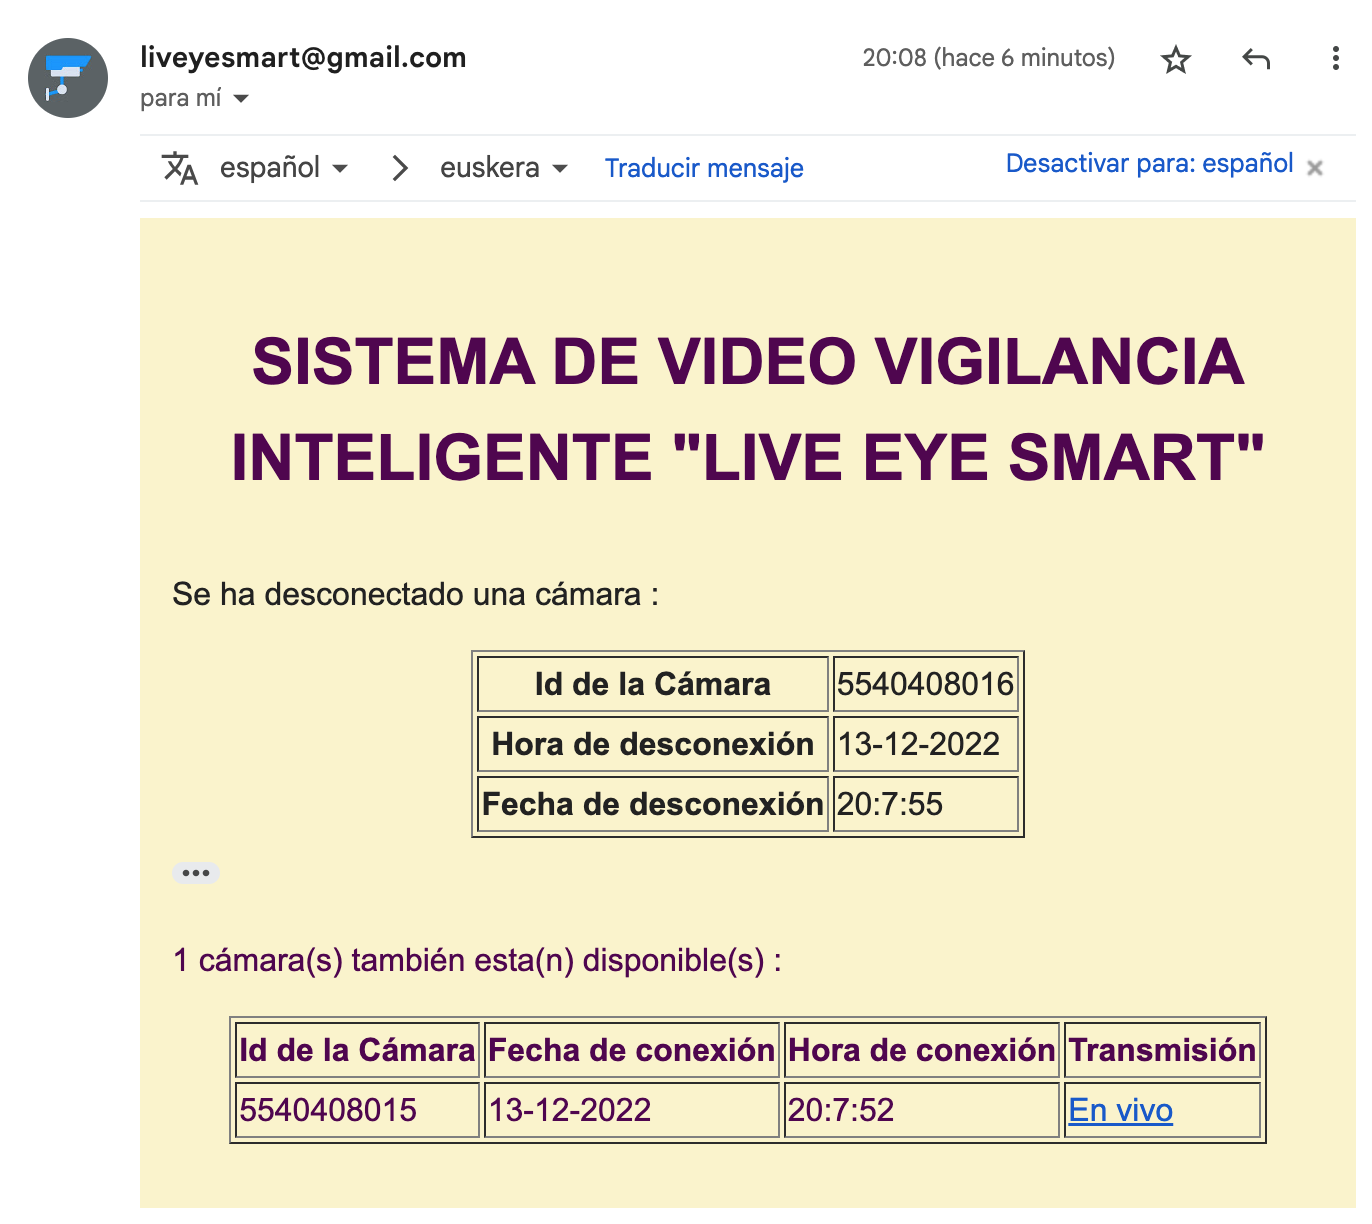
\includegraphics[width=10cm]{img/capitulo_6/mail3.png}
    \end{center}
    \begin{center}
        \caption{Notificación por correo - Cámara desconectada de varias.}
        Fuente : Elaboración propia
    \end{center}
\end{figure}

\section{Prueba de detección de fuego y notificación inmediata}

En la siguiente tabla se describe la prueba realizada sobre el detector:\\

\begin{table}[H]
    \caption{Detalle de prueba de detector de fuego}
    \begin{center}
        \begin{tabular}{|>{\centering}p{0.3\textwidth}|m{0.6\textwidth}<{\centering}|} 
            \hline
            \textbf{Título de la prueba} & Detector de fuego identifica incidencia \\
            \hline
            \textbf{Descripción} & El servidor se encuentra en ejecución y el proceso de identificación de fuego detecta una incidencia.\\
            \hline
            \textbf{Comportamiento obtenido} & 
            \begin{itemize}
                \item El servidor captura los fotogramas como prueba de la incidencia.
                \item El servidor notifica al usuario por medio de correo electronico.
                \item La notificación provee información sobre la fecha y hora de la incidencia, compartiendo el enlace para la transmisión en vivo.
            \end{itemize} \\ 
            \hline
            \textbf{Estado de prueba} & Exitoso \\
            \hline
        \end{tabular}
    \end{center}
    \begin{center}
        Fuente: Elaboración propia.
    \end{center}
\end{table}

A continuación se muestra las capturas del comportamiento esperado:

\begin{figure}[H]
    \begin{center}
        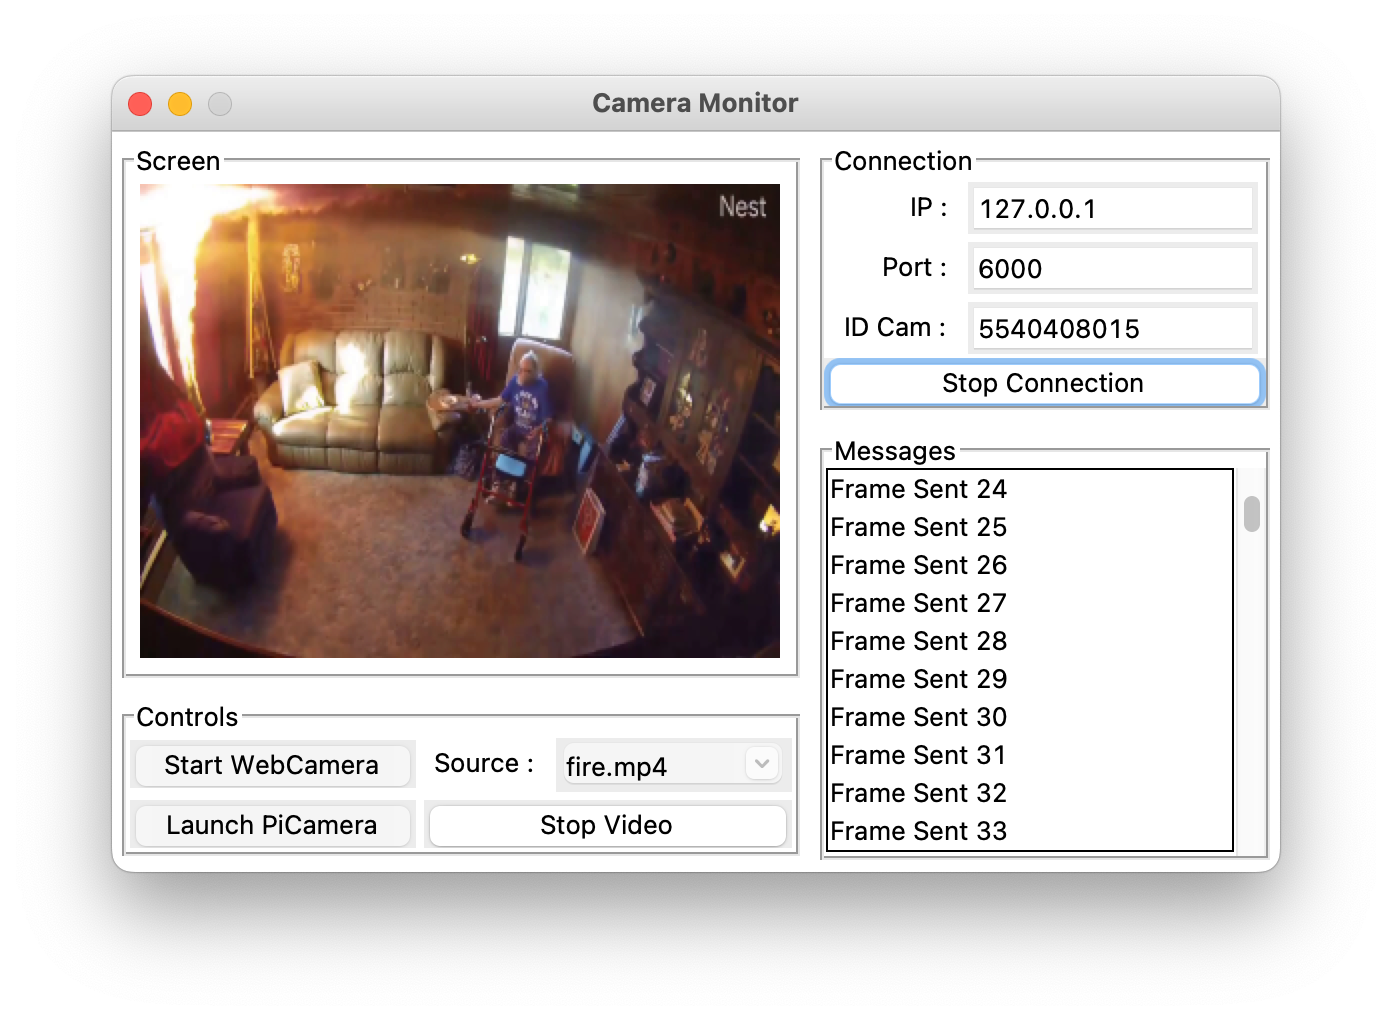
\includegraphics[width=11cm]{img/capitulo_6/fire.png}
    \end{center}
    \begin{center}
        \caption{Presencia de fuego en la escena.}
        Fuente : Elaboración propia
    \end{center}
\end{figure}

\begin{figure}[H]
    \begin{center}
        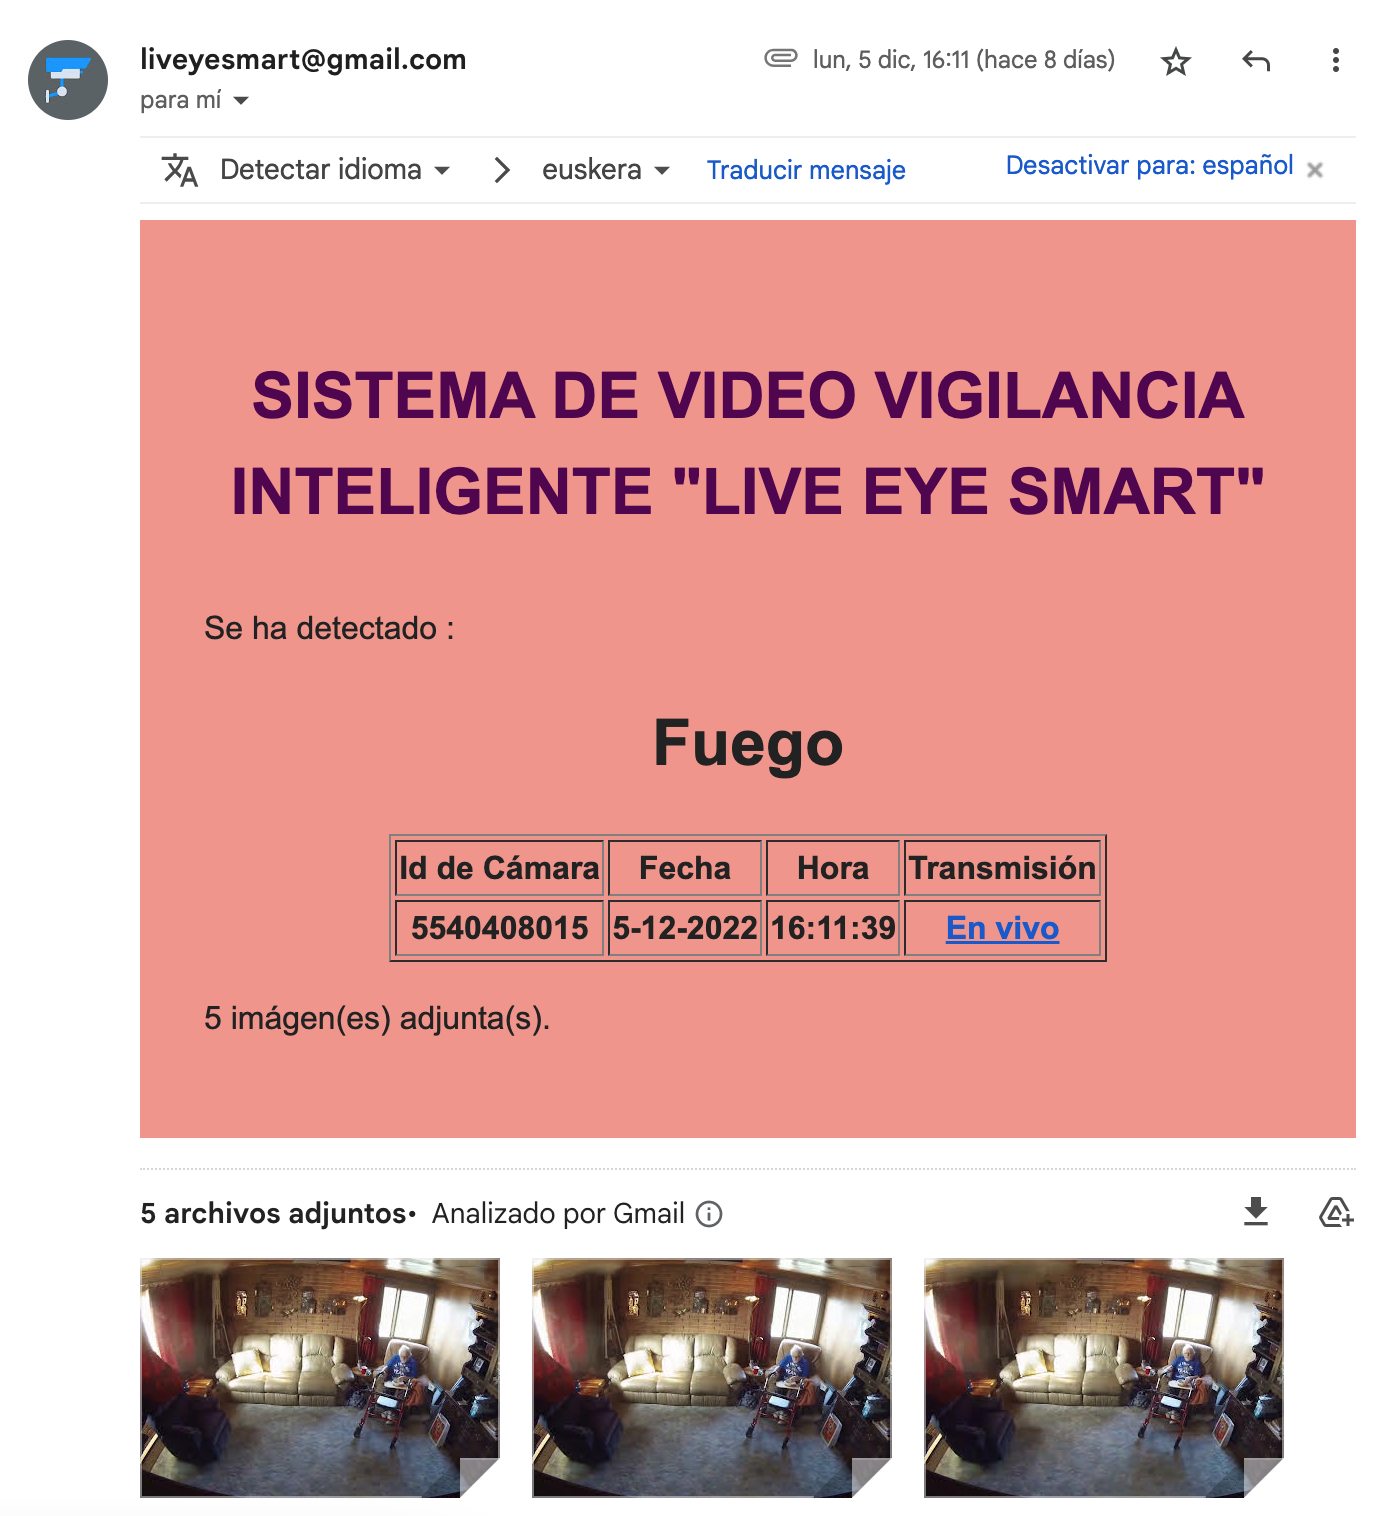
\includegraphics[width=10cm]{img/capitulo_6/mail_fire.png}
    \end{center}
    \begin{center}
        \caption{Detalle de notificación por correo electrónico - Alerta de fuego.}
        Fuente : Elaboración propia
    \end{center}
\end{figure}

\section{Prueba de detección de silueta humana y notificación inmediata}

En la siguiente tabla se describe la prueba realizada sobre el detector:

\begin{table}[H]
    \caption{Detalle de prueba de detector de silueta humana}
    \begin{center}
        \begin{tabular}{|>{\centering}p{0.3\textwidth}|m{0.6\textwidth}<{\centering}|} 
            \hline
            \textbf{Título de la prueba} & Detector de silueta humana identifica incidencia \\
            \hline
            \textbf{Descripción} & El servidor se encuentra en ejecución y el proceso de identificación de silueta humana detecta una incidencia.\\
            \hline
            \textbf{Comportamiento obtenido} & 
            \begin{itemize}
                \item El servidor captura los fotogramas como prueba de la incidencia.
                \item El servidor notifica al usuario por medio de correo electronico.
                \item La notificación provee información sobre la fecha y hora de la incidencia, compartiendo el enlace para la transmisión en vivo.
            \end{itemize} \\ 
            \hline
            \textbf{Estado de prueba} & Exitoso \\
            \hline
        \end{tabular}
    \end{center}
    \begin{center}
        Fuente: Elaboración propia.
    \end{center}
\end{table}

A continuación se muestra las capturas del comportamiento esperado:

\begin{figure}[H]
    \begin{center}
        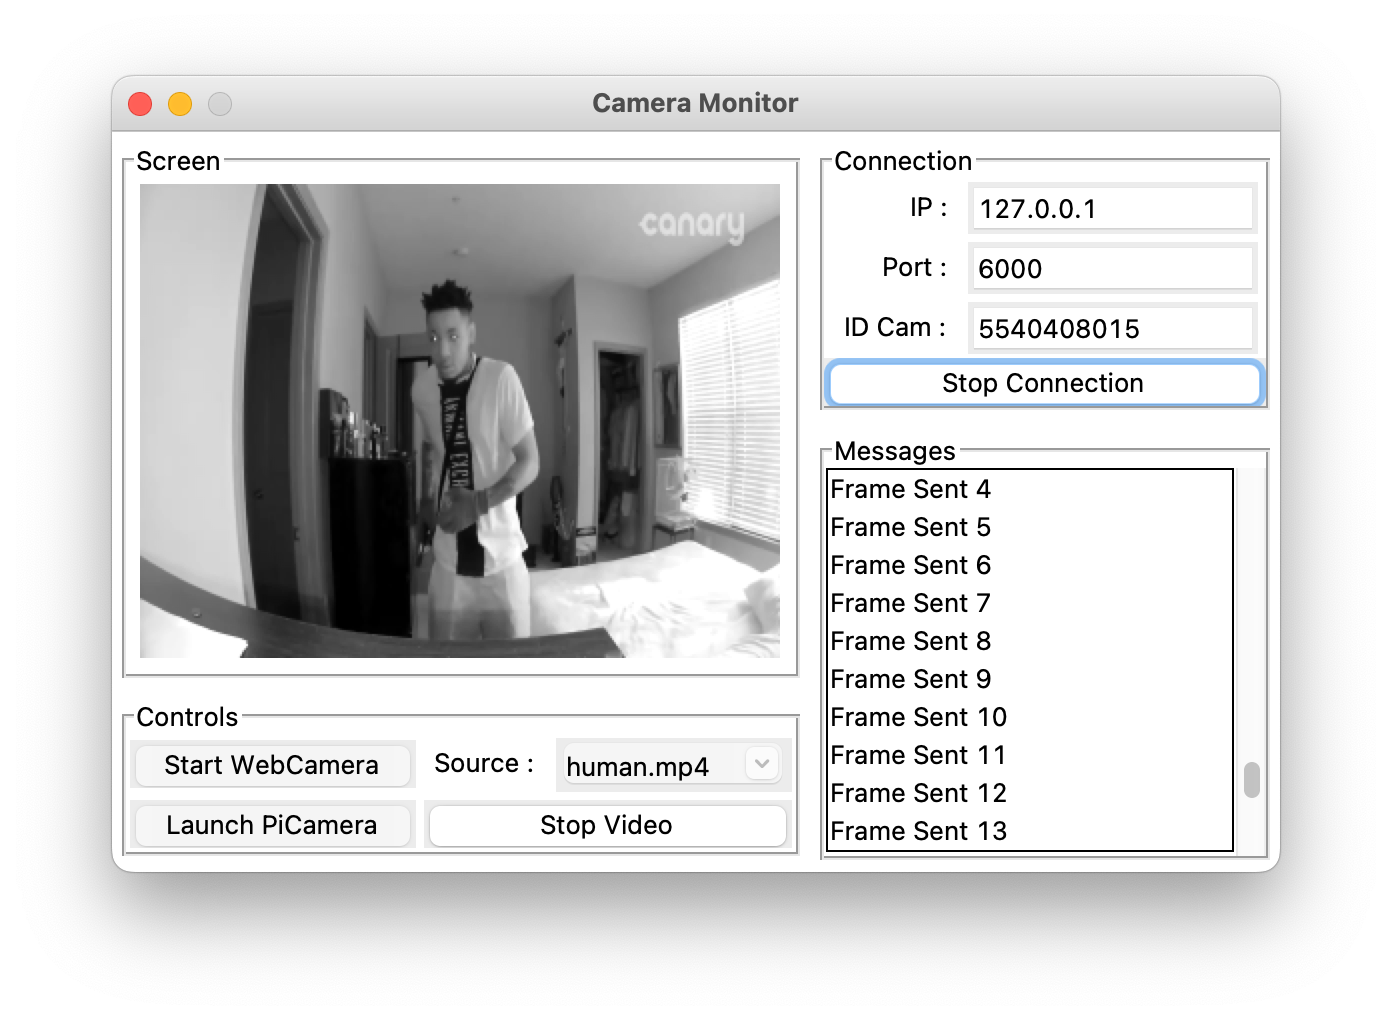
\includegraphics[width=12cm]{img/capitulo_6/human.png}
    \end{center}
    \begin{center}
        \caption{Visualización en módulo de cámaras - Presencia de intruso en la escena.}
        Fuente : Elaboración propia
    \end{center}
\end{figure}

\begin{figure}[H]
    \begin{center}
        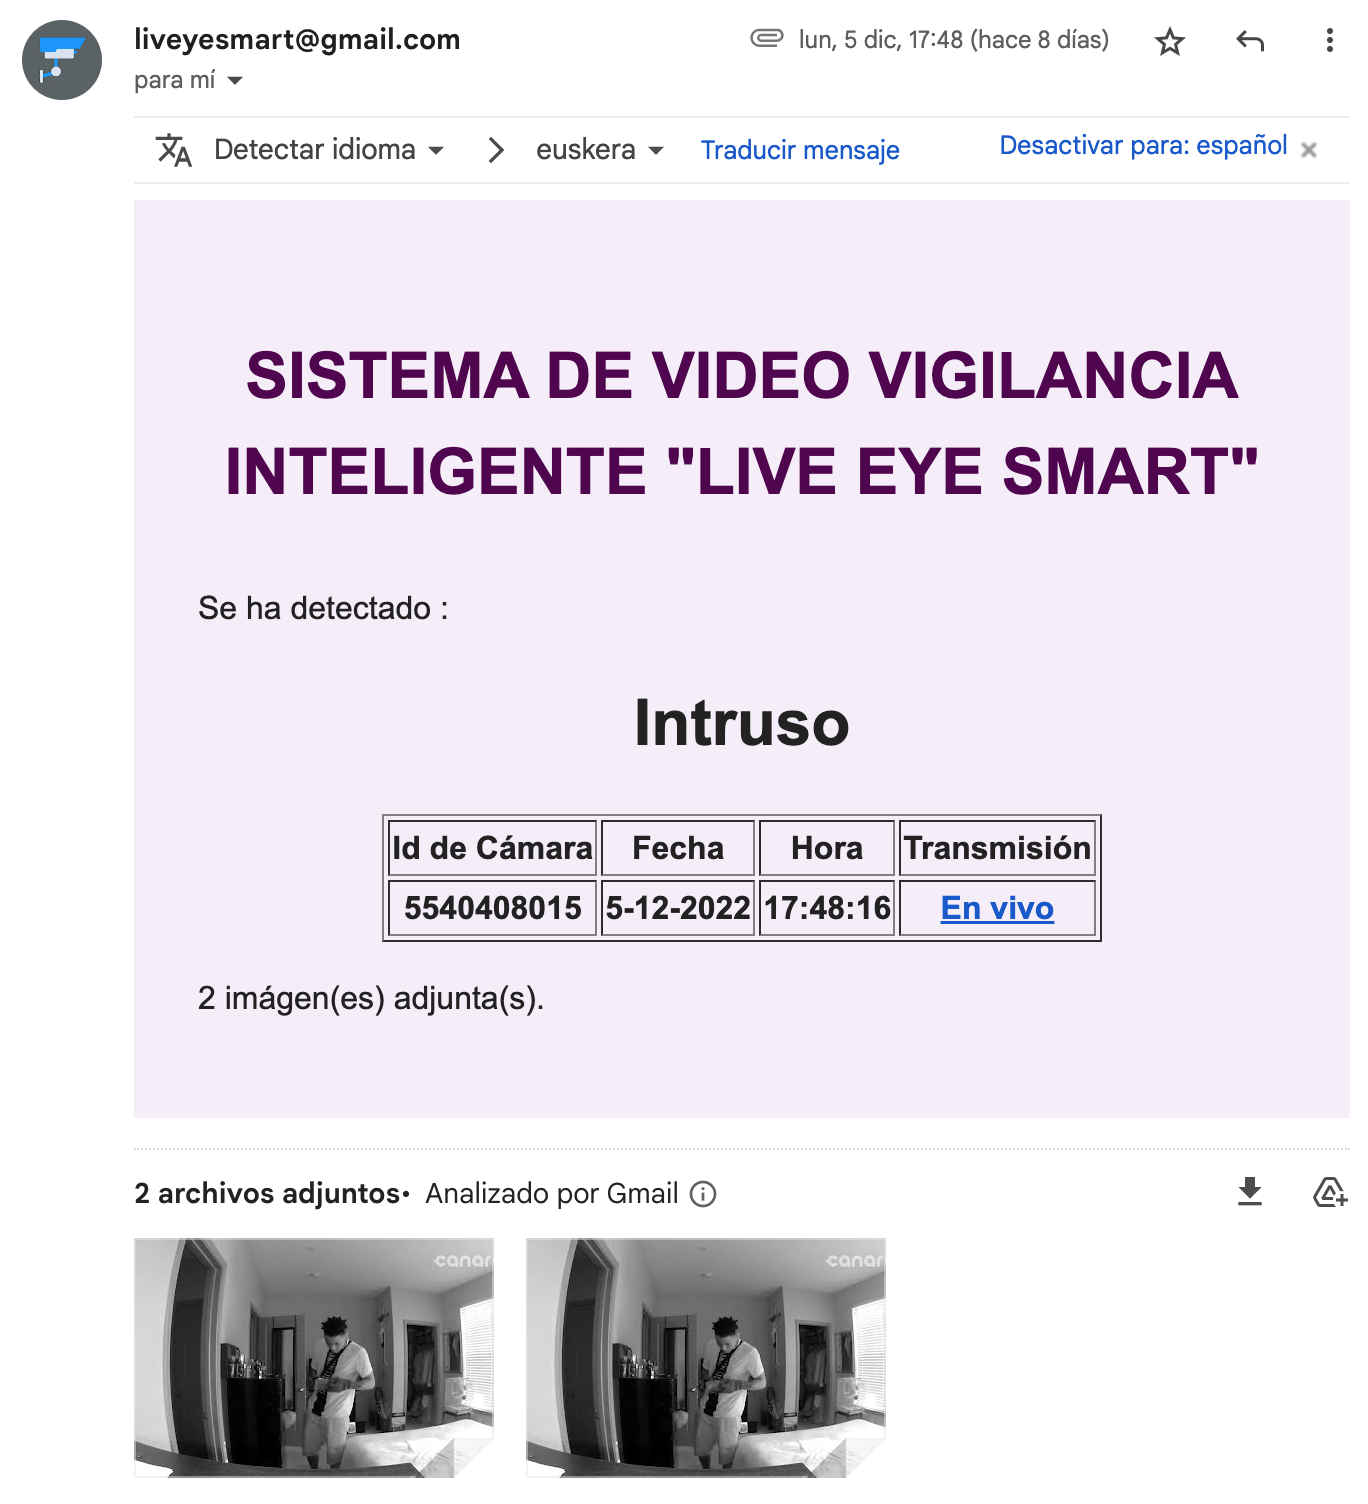
\includegraphics[width=8cm]{img/capitulo_6/mail_human.png}
    \end{center}
    \begin{center}
        \caption{Detalle de notificación por correo electrónico - Alerta de intruso.}
        Fuente : Elaboración propia
    \end{center}
\end{figure}


\section{Prueba de detección de movimiento y notificación inmediata}

En la siguiente tabla se describe la prueba realizada sobre el detector:\\

\begin{table}[H]
    \caption{Detalle de prueba de detector de movimiento}
    \begin{center}
        \begin{tabular}{|>{\centering}p{0.3\textwidth}|m{0.6\textwidth}<{\centering}|} 
            \hline
            \textbf{Título de la prueba} & Detector de movimiento identifica incidencia \\
            \hline
            \textbf{Descripción} & El servidor se encuentra en ejecución y el proceso de identificación de silueta humana detecta una incidencia.\\
            \hline
            \textbf{Comportamiento obtenido} & 
            \begin{itemize}
                \item El servidor captura los fotogramas como prueba de la incidencia.
                \item El servidor notifica al usuario por medio de correo electronico.
                \item La notificación provee información sobre la fecha y hora de la incidencia, compartiendo el enlace para la transmisión en vivo.
            \end{itemize} \\ 
            \hline
            \textbf{Estado de prueba} & Exitoso \\
            \hline
        \end{tabular}
    \end{center}
    \begin{center}
        Fuente: Elaboración propia.
    \end{center}
\end{table}

A continuación se muestra las capturas del comportamiento esperado:

\begin{figure}[H]
    \begin{center}
        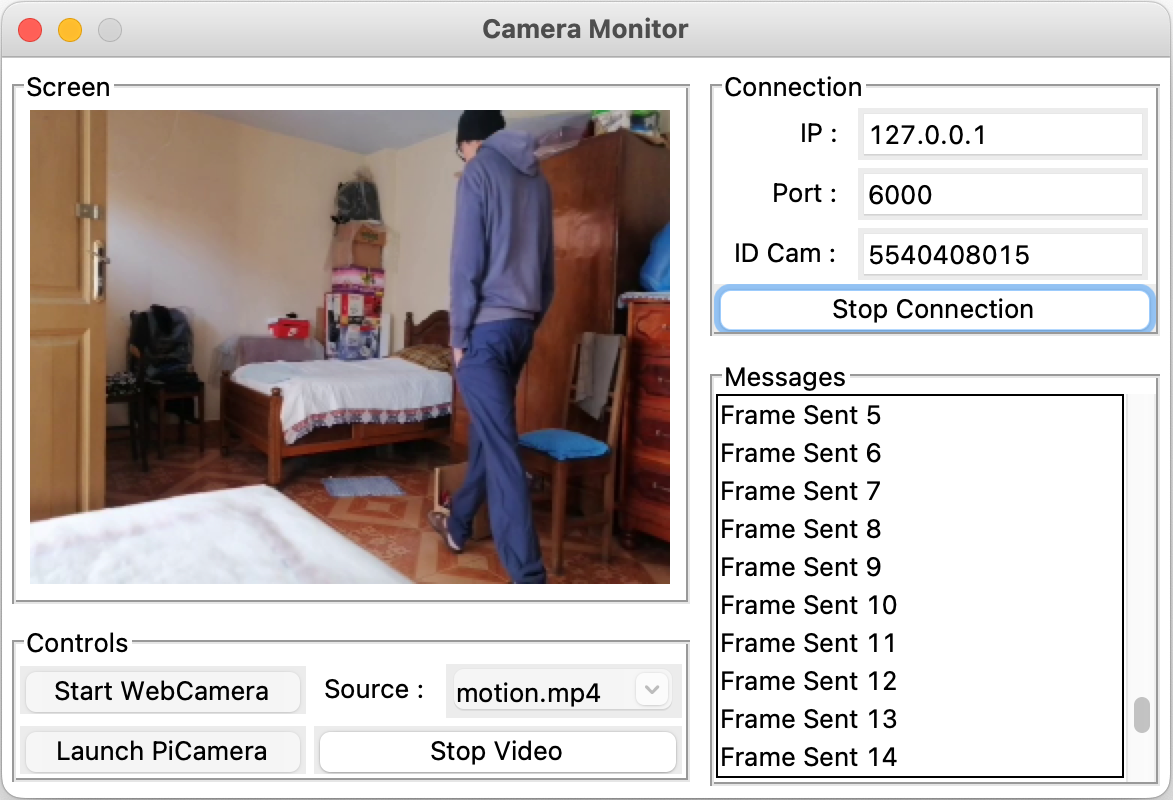
\includegraphics[width=11cm]{img/capitulo_6/motion.png}
    \end{center}
    \begin{center}
        \caption{Visualización en módulo de cámaras - Movimiento.}
        Fuente : Elaboración propia
    \end{center}
\end{figure}

\begin{figure}[H]
    \begin{center}
        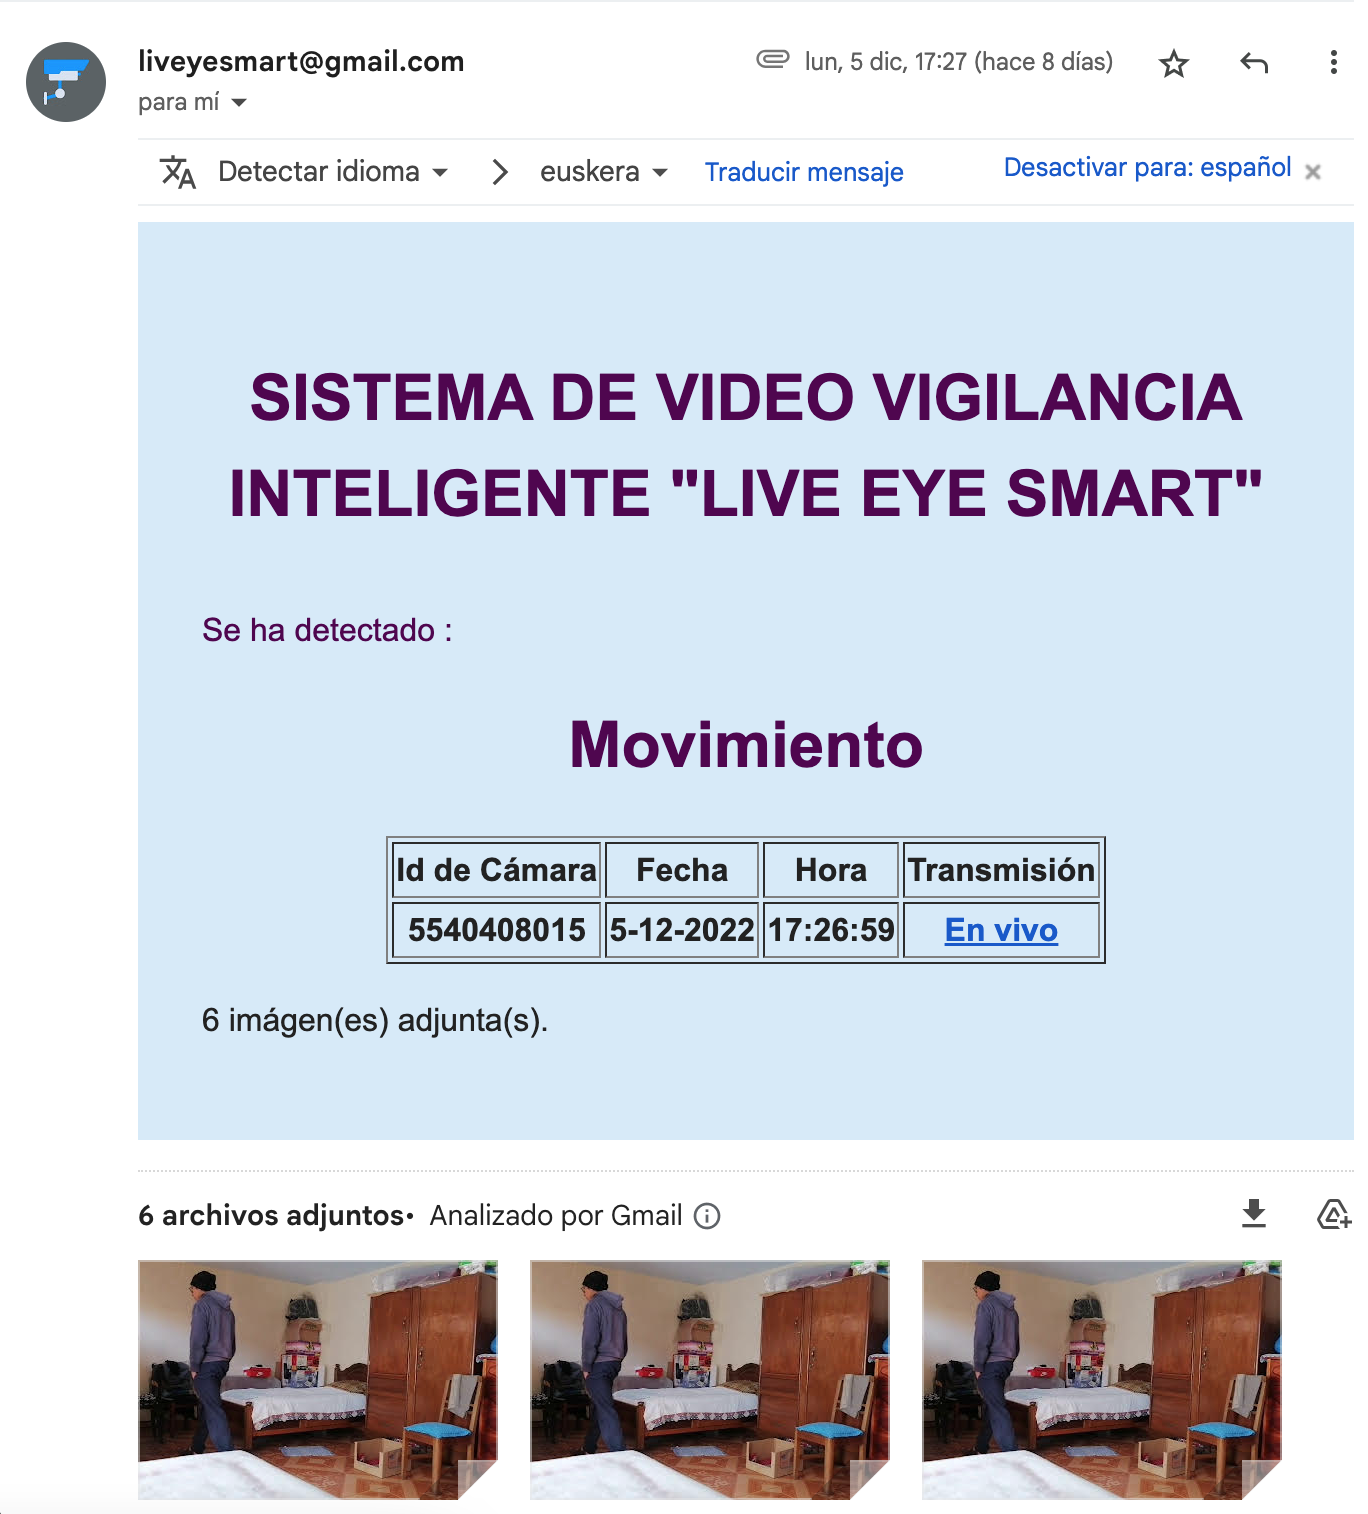
\includegraphics[width=9cm]{img/capitulo_6/mail_motion.png}
    \end{center}
    \begin{center}
        \caption{Detalle de notificación por correo electrónico - Alerta de movimiento.}
        Fuente : Elaboración propia
    \end{center}
\end{figure}

\section{Prueba de transmisión de video en vivo}

En la siguiente tabla se describe la prueba realizada:\\

\begin{table}[H]
    \caption{Detalle de prueba de la transmisión de video en vivo.}
    \begin{center}
        \begin{tabular}{|>{\centering}p{0.3\textwidth}|m{0.6\textwidth}<{\centering}|} 
            \hline
            \textbf{Título de la prueba} & Transmisión de video\\
            \hline
            \textbf{Descripción} & El servidor se encuentra en ejecución y una instancia del módulo de cámaras se conecta al servidor. El usuario ingresa al enlace que le llega en la notificación para la transmisión de video en vivo.\\
            \hline
            \textbf{Comportamiento obtenido} & 
            \begin{itemize}
                \item El servidor registra la conexión y lo muestra en consola.
                \item El servidor comienza con la decodificación video en streaming.
                \item La notificación provee información del enlace para su transmisión en vivo.
                \item La transmisión se visualiza en un reproductor de video adaptativo en el navegador.
            \end{itemize} \\ 
            \hline
            \textbf{Estado de prueba} & Exitoso \\
            \hline
        \end{tabular}
    \end{center}
    \begin{center}
        Fuente: Elaboración propia.
    \end{center}
\end{table}

A continuación se muestra las capturas del comportamiento esperado:\\

\begin{figure}[H]
    \begin{center}
        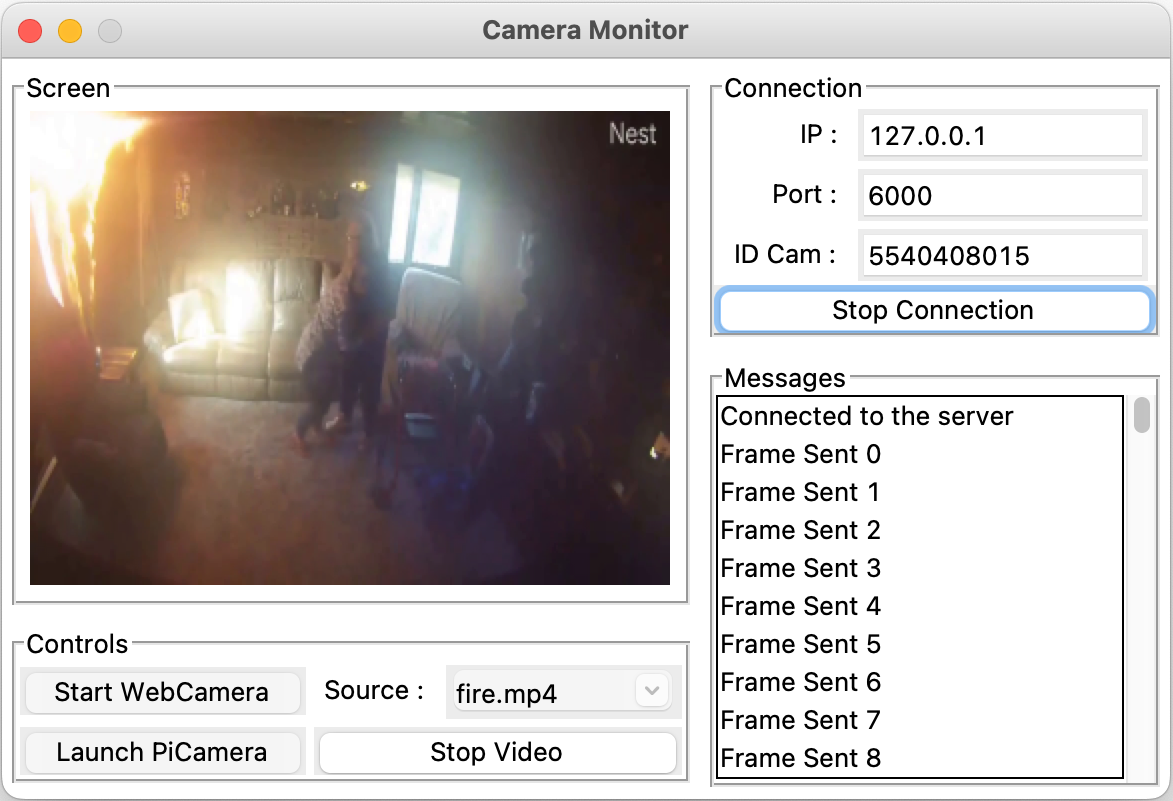
\includegraphics[width=12cm]{img/capitulo_6/stream.png}
    \end{center}
    \begin{center}
        \caption{Visualización en módulo de cámaras.}
        Fuente : Elaboración propia
    \end{center}
\end{figure}

\begin{figure}[H]
    \begin{center}
        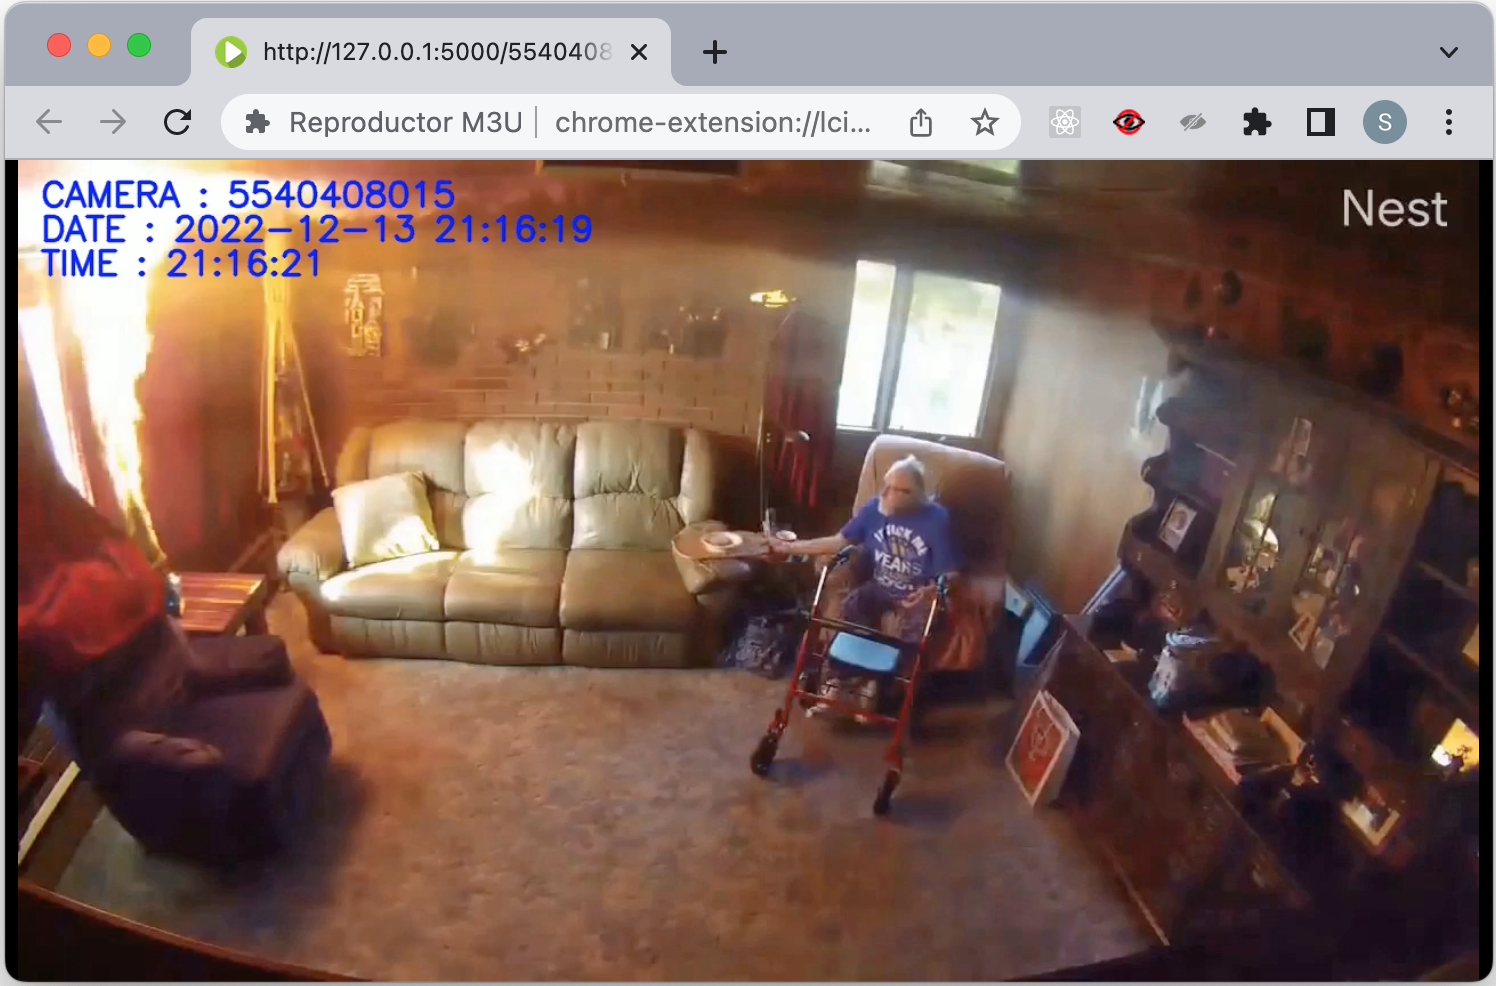
\includegraphics[width=15cm]{img/capitulo_6/stream_web.png}
    \end{center}
    \begin{center}
        \caption{Reproductor web de video en Streaming.}
        Fuente : Elaboración propia
    \end{center}
\end{figure}